% =========================================================================
% Compile with: pdflatex report.tex  (run twice for cross-references)
% Required: pdflatex, standard texlive packages.
%
% Figure: the report embeds "Processing_Pipeline.pdf" directly from
% the project root. The grffile package handles the spaces in the filename.
% =========================================================================
\documentclass[11pt,a4paper]{article}

\usepackage[utf8]{inputenc}
\usepackage[T1]{fontenc}
\usepackage[margin=2.3cm]{geometry}
\usepackage{graphicx}
\usepackage{grffile} % allow spaces in graphics filenames
\usepackage{booktabs}
\usepackage{amsmath}
\usepackage{xcolor}
\usepackage{listings}
\usepackage{hyperref}
\usepackage{caption}
\usepackage{enumitem}
\usepackage{microtype}

\hypersetup{colorlinks=true, linkcolor=blue, citecolor=blue, urlcolor=blue}

\lstset{
  basicstyle=\ttfamily\footnotesize,
  breaklines=true,
  frame=single,
  numbers=none,
  showstringspaces=false,
  xleftmargin=0.5em,
  xrightmargin=0.5em,
}

\title{Assignment 1 - Text Processing Fundamentals using MapReduce}
\author{Group 36 --- Data-Intensive Computing (194.048), TU Wien\\
        \small Schmidt Felix Rudolf, Trapuzzano Gianluca, Vani Marvi,
        Trumshi Fiona, Emon Md.~Emamul Hasan}
\date{April 28, 2026}

\begin{document}
\maketitle

\section{Introduction}

Identifying the most discriminative vocabulary of a document collection is a
recurring task in text mining: it powers feature selection for classification,
domain-specific dictionary construction, and exploratory analysis of large
review corpora.  In this assignment we apply the chi-square ($\chi^{2}$) test
of independence to the Amazon Reviews dataset to extract, for each of the
22~product categories, the 75 unigram terms most strongly associated with
that category.  The full corpus comprises about 78.8 million review records
distributed across an HDFS file of approximately 56~GB, which makes the
problem genuinely data-intensive and motivates a MapReduce solution.

The pipeline is implemented with the \texttt{mrjob} Python framework and
executed on the TU~Wien LBD Hadoop cluster (Hadoop~3.3.6, YARN). All
correctness and performance numbers reported here come from a single end-to-end
run on the full dataset that completed in 19~min~24~s of wall-clock time.

\section{Problem Overview}

\subsection*{Input and output}

The input is a line-delimited JSON file in which every record contains among other features a \texttt{category} field and a \texttt{reviewText} field. The required
output is a single text file with 23 lines:

\begin{itemize}[leftmargin=*,nosep]
  \item 22~category lines, sorted alphabetically by category name. Each line
        starts with the category name followed by 75 \texttt{word:chi2}
        tokens, sorted by descending $\chi^{2}$ score.
  \item 1 final line with the merged dictionary: the alphabetically sorted
        union of all words selected as top-75 in any category.
\end{itemize}

\subsection*{Chi-square statistic}

For each (term~$t$, category~$c$) pair we build a $2\times2$ contingency
table over the documents of the corpus:

\begin{center}
\begin{tabular}{lcc}
\toprule
            & in category $c$ & not in category $c$ \\
\midrule
contains $t$     & $A$ & $C$ \\
does not contain $t$ & $B$ & $D$ \\
\bottomrule
\end{tabular}
\end{center}

\noindent The values are derived from three aggregates:
$\textit{cat\_total}_c$ (documents in $c$),
$\textit{token\_total}_t$ (documents containing $t$ across all categories),
and $N$ (total documents):
\[
B = \textit{cat\_total}_c - A,\quad
C = \textit{token\_total}_t - A,\quad
D = N - \textit{cat\_total}_c - \textit{token\_total}_t + A.
\]
The score is then
\begin{equation}
\chi^{2}(t,c) \;=\;
\frac{N\,(A\,D - B\,C)^{2}}
     {\textit{token\_total}_t\,(N-\textit{token\_total}_t)\,
      \textit{cat\_total}_c\,(N-\textit{cat\_total}_c)}.
\label{eq:chi2}
\end{equation}

\subsection*{Document frequency, not term frequency}

A subtle but critical detail: $A$ is a \emph{document frequency}, i.e.\ the
number of documents in $c$ that contain $t$ at least once, not the number of
times $t$ occurs.  An implementation that emits one count per token
\emph{occurrence} would inflate $A$ and can even violate $A \le
\textit{cat\_total}_c$, breaking the contingency table.  Our mapper therefore
deduplicates tokens within each document before emission
(see~Section~\ref{sec:step1}).

\subsection*{Dataset characteristics (from cluster counters)}

The full run reports $N = 78{,}828{,}876$ reviews distributed over 22
categories. After preprocessing, the post-stopword vocabulary contains
roughly $6.2$~million distinct unigrams; the number of distinct $(c,t)$
pairs to be scored is approximately $12.19$~million. The fact that the
vocabulary grows sublinearly with collection size (Heaps' law) is what
makes a single-reducer pass over the post-aggregated stream tractable at
this scale; we return to this point in the discussion.

\section{Methodology}

\subsection{Pipeline overview}

Figure~\ref{fig:pipeline} shows the conceptual pipeline.  The
implementation realises it as four \texttt{MRStep}s, which \texttt{mrjob}
submits as a chained sequence of four Hadoop streaming jobs sharing one
temporary HDFS directory for the intermediate outputs.  Phase~3 of the
figure corresponds to two physical MRSteps in the code: one to aggregate
token totals across categories (MRStep~2) and one to compute and rank
$\chi^{2}$ scores (MRStep~3); Phase~4 of the figure corresponds to
MRStep~4 (final assembly).

\begin{figure}[h]
  \centering
  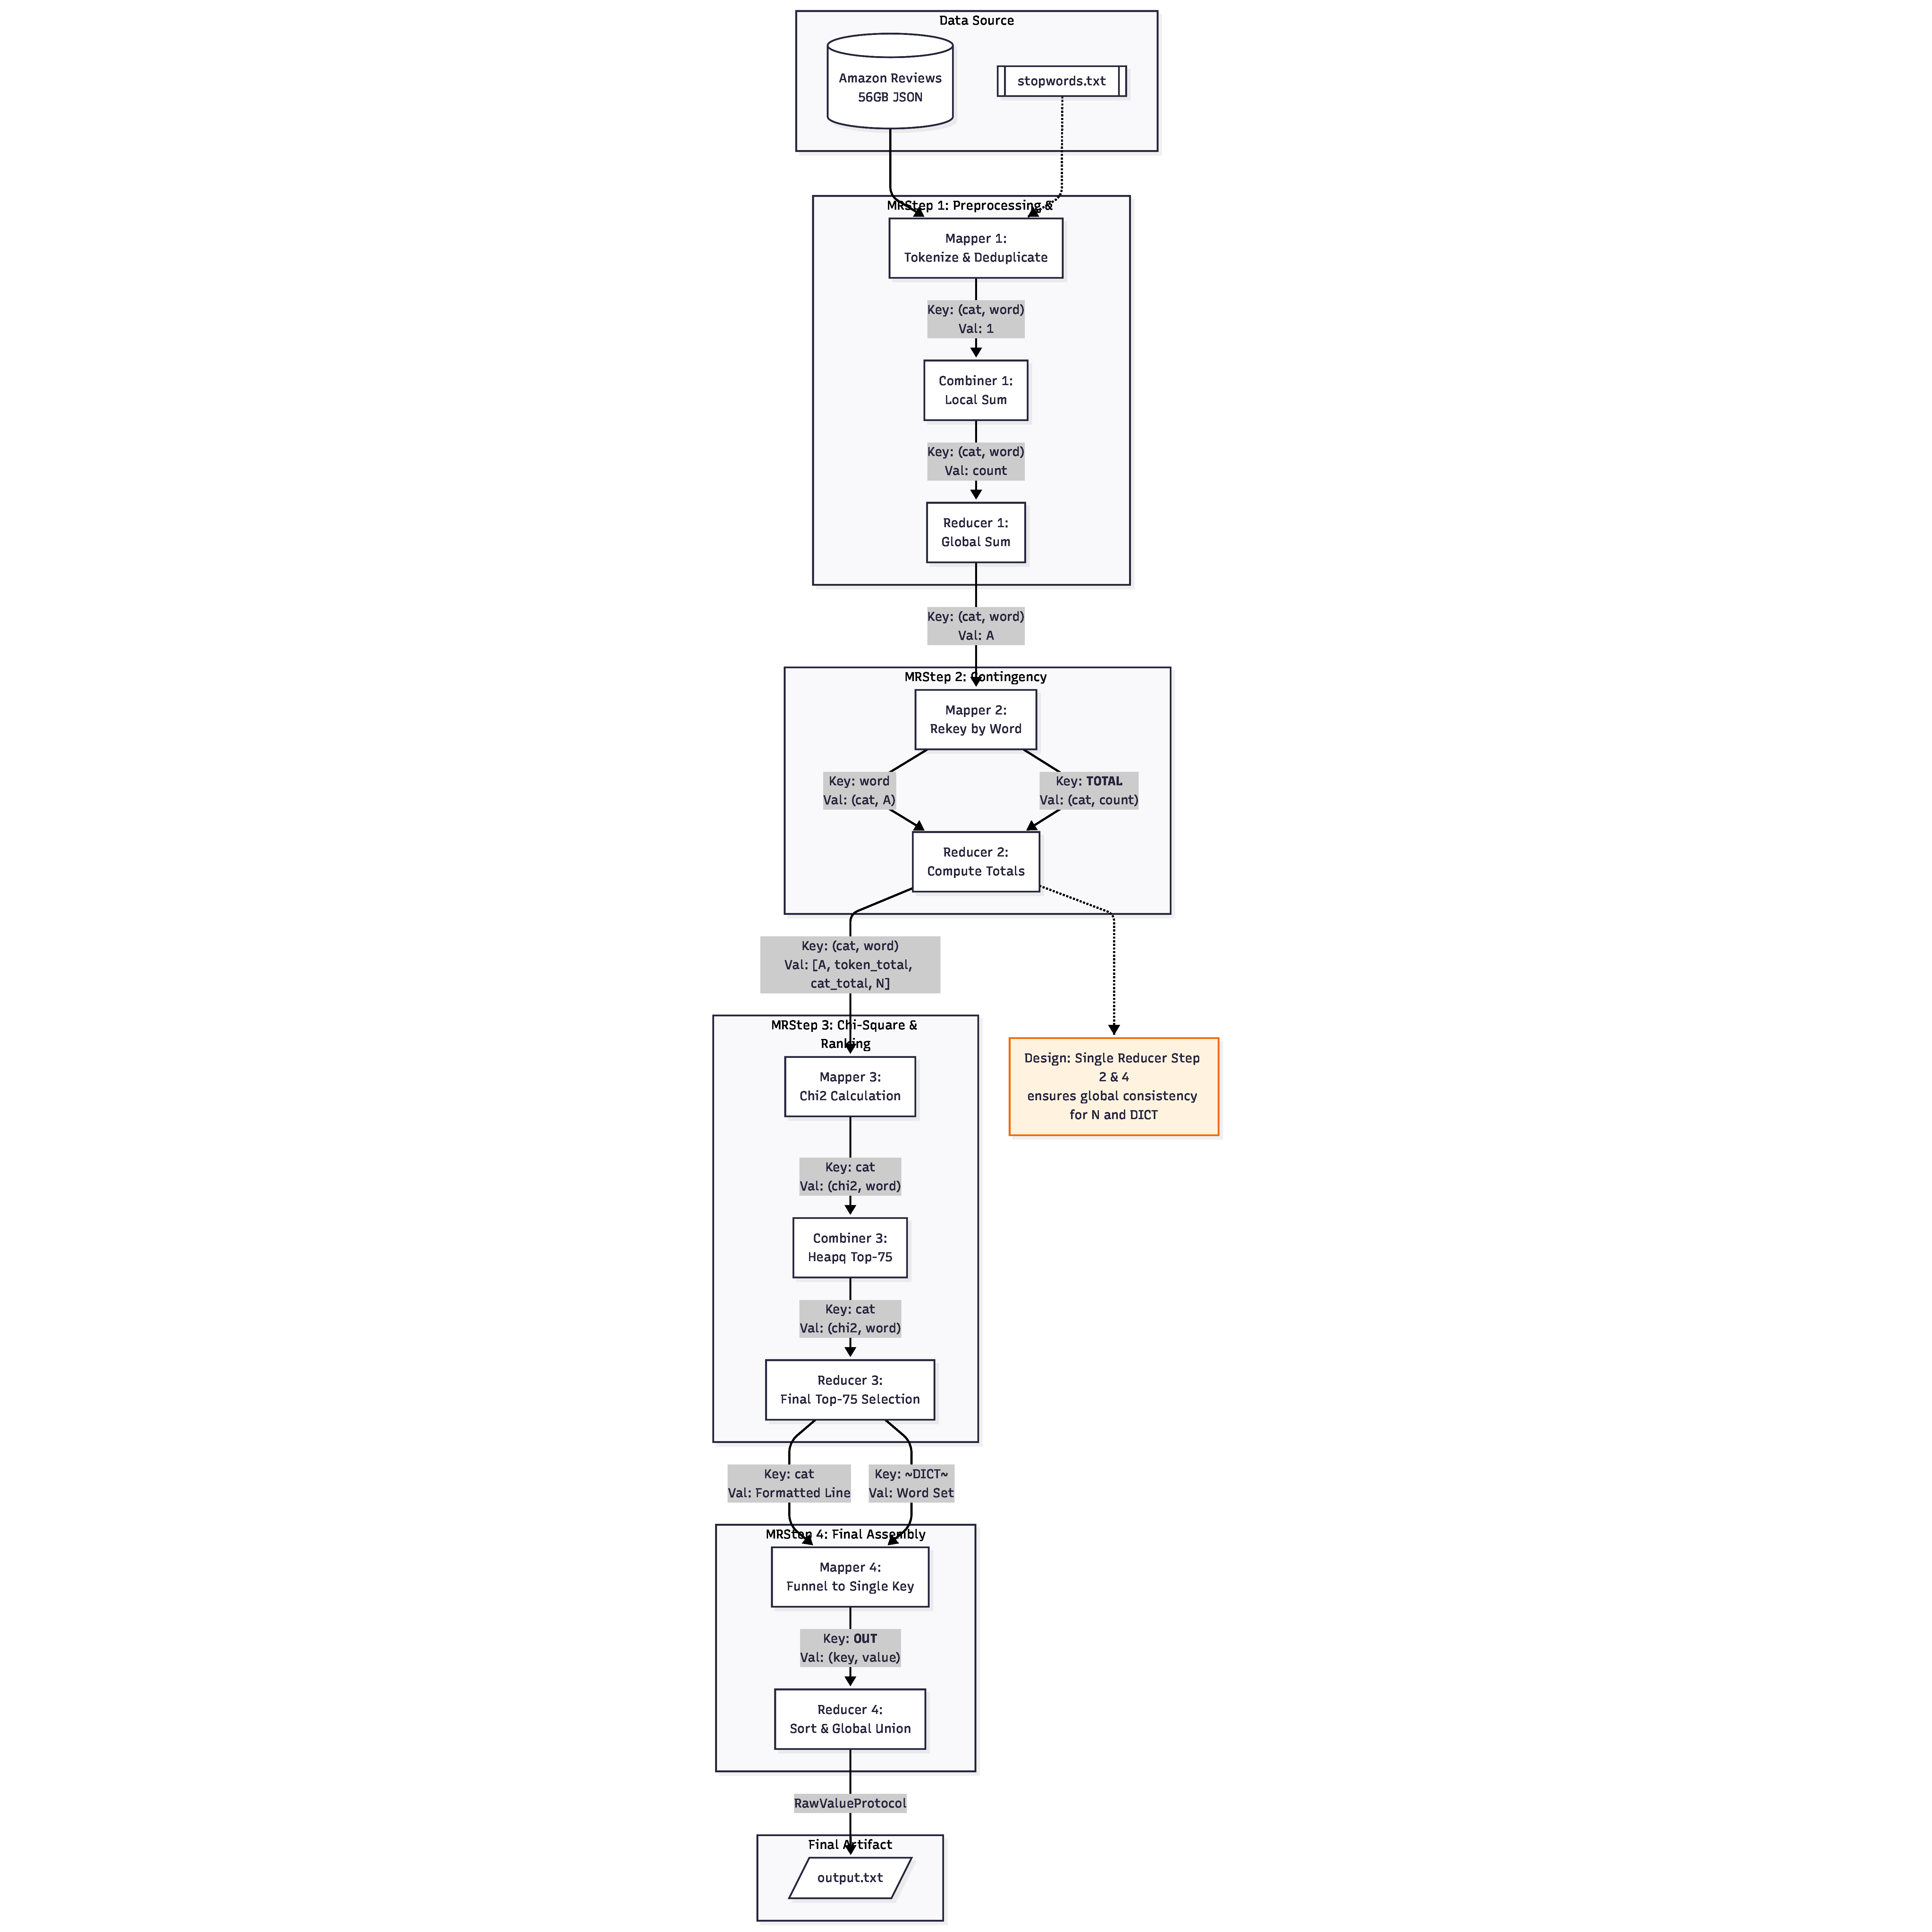
\includegraphics[width=\textwidth,keepaspectratio]{Processing_Pipeline.pdf}
  \caption{Conceptual pipeline.  Phase~0 loads stopwords once per mapper
  task (\texttt{mapper\_init}). Phase~1 does the heavy lifting on the raw
  56~GB input. Phase~2 is \texttt{mrjob}'s internal shuffle.  Phase~3
  computes the contingency-table aggregates, evaluates~$\chi^{2}$, and
  selects the top~75 per category. Phase~4 emits the 22~category lines and
  the merged dictionary in the required \texttt{output.txt} format.}
  \label{fig:pipeline}
\end{figure}

\subsection{MRStep~1 --- Preprocessing and document-frequency counting}
\label{sec:step1}

\textbf{Mapper.}  For every input record, the JSON line is parsed with
\texttt{ujson} (falling back to the standard \texttt{json} module if
\texttt{ujson} is not installed on the cluster image).  The
\texttt{reviewText} field is lower-cased and split on a single regular
expression that treats all required punctuation, whitespace, tabs and digits
as delimiters in one pass.  Each token is filtered against the stopword set
(loaded once in \texttt{mapper\_init}) and the minimum-length rule
($|w|>1$).  The surviving tokens are inserted into a per-document
\emph{set}, and only \emph{after} the document is fully tokenised does the
mapper emit one record per distinct token:

\begin{lstlisting}[language=Python]
seen = set()
for word in self.splitting_on.split(review_text):
    if word and word not in self.stopwords and len(word) > 1:
        seen.add(word)
for word in seen:
    yield (category, word), 1
yield (category, '__TOTAL__'), 1
\end{lstlisting}

The deduplication ensures that downstream $A$ values are document
frequencies. The extra \texttt{(category, '\_\_TOTAL\_\_')} record carries
the per-category document count needed to derive $\textit{cat\_total}$ and
$N$ in MRStep~2.

\textbf{Combiner.}  An in-mapper combiner sums counts locally before they
are shuffled to the reducer. On the full run the combiner reduces
2.34~billion intermediate records to 144~million, a shrink factor of~16$\times$
that is essential to keep the shuffle volume manageable
(Table~\ref{tab:counters}).

\textbf{Reducer.}  A single reducer sums counts globally (we did not
override the default reducer count for this step, since the heavy lifting
is already absorbed by the combiner). Its output is $12.19$~million
$((c,w)\!\to\!\textit{count})$ records together with 22 records of the form
$((c,\texttt{\_\_TOTAL\_\_})\!\to\!\textit{cat\_total})$.

\subsection{MRStep~2 --- Rekey and token-total computation}

To compute $\textit{token\_total}_t = \sum_{c} A_{c,t}$, all per-category
counts of the same token must arrive at the same reducer task. The mapper
therefore rekeys the stream by token:

\begin{lstlisting}[language=Python]
def mapper_2(self, key, count):
    cat, word = key
    if word == '__TOTAL__':
        yield '__TOTAL__', (cat, count)
    else:
        yield word, (cat, count)
\end{lstlisting}

The reducer accumulates the 22~\texttt{\_\_TOTAL\_\_} records into a
dictionary, derives $N$, and then for each token computes
$\textit{token\_total}$ on the fly and emits one record per category in
which the token appears, carrying the four values needed for $\chi^{2}$:

\begin{lstlisting}[language=Python]
yield (cat, word), [A, token_total, cat_total, self.N]
\end{lstlisting}

This step is configured with \verb|jobconf={'mapreduce.job.reduces': '1'}|
because the \texttt{\_\_TOTAL\_\_} aggregates have to be visible to
\emph{every} word reducer call. With Hadoop's default hash partitioning,
the single \texttt{\_\_TOTAL\_\_} key would otherwise be assigned to one
specific reducer task only, leaving the other tasks (which receive
disjoint subsets of the words) without the \textit{cat\_total} and $N$
values they need to populate the contingency table.  Forcing a single
reducer guarantees that every word and every \texttt{\_\_TOTAL\_\_}
record arrive at the same task; the JSON-encoded key
\texttt{"\_\_TOTAL\_\_"} sorts before any lower-case word, so the
dictionary is fully populated by the time the first word record is
processed. The trade-off is sequential reduce work; we quantify its
actual cost in Section~\ref{sec:results} and discuss a parallelisable
alternative in Section~\ref{sec:conclusions}.

\subsection{MRStep~3 --- Chi-square, top-75, partial dictionary}

The mapper computes Equation~\ref{eq:chi2} directly and rekeys by
category. Records with a degenerate denominator (e.g.\ a token appearing in
every document, or an empty category) are dropped.

\textbf{Bounded top-$k$ with \texttt{heapq}.}  The combiner and reducer
both use \texttt{heapq.nsmallest(75, values, key=lambda x: (-x[0], x[1]))}
to pick the local top~75 by $-\chi^{2}$ with alphabetic tie-break. This is
linear in the number of values and uses $\mathcal{O}(75)$ extra memory,
unlike a full \texttt{sorted()}.  The combiner alone shrinks this
step's shuffle from $12.18$~million records to $18\,150$ (a factor of
$670\times$, see Table~\ref{tab:counters}); without the combiner the
single Step-3 reducer would be the dominant bottleneck.

\textbf{Merged dictionary.}  Every reducer call adds the selected
words to a shared \texttt{self.dict\_words} set; \texttt{reducer\_final}
emits the partial dictionary under the sentinel key \texttt{\textasciitilde
DICT\textasciitilde}.

\subsection{MRStep~4 --- Final assembly}

The mapper funnels every Step-3 record under one synthetic key
(\texttt{\_\_OUT\_\_}), which forces all of them into a single reducer
call (the data volume is~23 records, so this is essentially free). The
reducer separates category lines from \texttt{\textasciitilde DICT\textasciitilde}
partials, sorts the categories alphabetically, unions the partials into the
final dictionary line, and emits everything via
\texttt{RawValueProtocol} so that the \texttt{mrjob} stdout is already in
the required \texttt{output.txt} format --- no post-processing script is
needed.

\subsection{Cluster results}
\label{sec:results}

The job was submitted to the LBD cluster with

\begin{lstlisting}[language=bash]
time python main.py \
  --hadoop-streaming-jar /usr/lib/hadoop/tools/lib/hadoop-streaming-3.3.6.jar \
  -r hadoop --upload-file stopwords.txt \
  hdfs:///dic_shared/amazon-reviews/full/reviewscombined.json \
  > output.txt 2> log.txt
\end{lstlisting}

and finished in \textbf{19~min~24~s} wall-clock time
(real~19m24.763s).  Table~\ref{tab:counters} summarises the
per-step Hadoop counters extracted from \texttt{log.txt}.

\begin{table}[h]
\centering
\small
\begin{tabular}{lrrrrr}
\toprule
Step & Map in & Map out & Combiner shrink & Reduce in/out & Reduce time \\
\midrule
1 & 78\,828\,876 & 2\,214\,174\,909 & $2.34\text{B}\!\to\!144\text{M}$ ($16\times$) & 21.4\,M / 12.2\,M & 597\,s \\
2 & 12\,189\,683 & 12\,189\,683    & ---                                & 12.2\,M / 12.2\,M & 172\,s \\
3 & 12\,175\,531 & 12\,175\,531    & $12.2\text{M}\!\to\!18\text{k}$ ($670\times$) & 18\,150 / 23 &   5\,s \\
4 &           23 &            23  & ---                                &     23 / 23  &   5\,s \\
\bottomrule
\end{tabular}
\caption{Per-step Hadoop counters for the full-dataset run. Combiner shrink
is reported only where a combiner is configured. Reduce time is the total
time spent in reduce tasks for the step (each step launched exactly one
reducer).}
\label{tab:counters}
\end{table}

\textbf{Splits and parallelism.} MRStep~1 was split into 435~map tasks
(launched~446, 11 killed); MRSteps 2--4 used 3, 9 and 2~map tasks
respectively. The total accumulated map CPU time was about 23.6~hours,
distributed across the cluster's available containers; the wall-clock map
phase of MRStep~1 fitted within the run because YARN scheduled roughly two
hundred concurrent map containers. The reducer side is, by contrast,
sequential: each step launched exactly one reducer task, so the
$\sim$13~minutes of total reduce time (Table~\ref{tab:counters}) lies on
the wall-clock critical path.

\textbf{Data reduction.}  The 56~GB input is reduced to 395~MB after
MRStep~1, a 147$\times$ reduction driven by the combiner. By the end of
MRStep~3 the relevant data is only 42~kB (Step~3 \texttt{Bytes Written});
the final \texttt{output.txt} is 41.97~kB.

\section{Conclusions}
\label{sec:conclusions}

The pipeline produces the required output and processes the full 56~GB
corpus in under 20~minutes wall-clock time, which was the desired outcome. Three design choices
contributed most to this result:

\begin{enumerate}[leftmargin=*,nosep]
\item \textbf{Document-frequency deduplication in the mapper}, which
      keeps the chi-square contingency table well-formed.
\item \textbf{Combiners on Steps~1 and~3}, both of which reduce shuffle
      volume by more than an order of magnitude (16$\times$ and 670$\times$).
      In particular, the bounded top-$k$ combiner in Step~3 turns
      a potentially expensive global sort into a linear-time selection
      with constant per-mapper memory.
\item \textbf{Output-side simplifications}: \texttt{RawValueProtocol} on
      the last step removes the need for a separate formatting script,
      and the single-key funnel in Step~4 keeps the final assembly
      deterministic across multiple reducers.
\end{enumerate}

The principal limitation is that every step launched exactly one reducer
task, putting the entire reduce phase on the sequential critical path
(roughly 13~minutes out of 19~min~24~s wall-clock). Two distinct
sub-issues are worth separating.

\textbf{(i) MRStep~2 is forced single-reducer} by the
\texttt{\_\_TOTAL\_\_} broadcast pattern. At our scale this only cost
$\sim$3~minutes thanks to Heaps' law: the post-aggregation stream is
bounded by the vocabulary, not by the raw review count.  For
substantially larger corpora the constraint would become a hard
bottleneck, and the canonical refactor is the \emph{distributed-cache /
side-input pattern}: a tiny preceding job materialises the per-category
totals into a small file, the main job loads that file via
\texttt{--upload-file} in \texttt{mapper\_init}, and the
\texttt{\_\_TOTAL\_\_} plumbing disappears entirely. MRStep~2 then
becomes embarrassingly parallel across an arbitrary number of reducers.

\textbf{(ii) MRStep~1 used a single reducer by default.} Unlike MRStep~2
this is not a correctness requirement --- summing $((c,w),\textit{count})$
keys is associative and partitionable --- so the step could be split
across $R$ reducers simply by setting \texttt{mapreduce.job.reduces}
explicitly. With $R = 8$ the $\sim$10-minute reduce phase of MRStep~1
would shrink to roughly 1.5~minutes, which alone would push the total
run-time well below 10~minutes. We did not implement either refactor
here because the current 19-minute run already comfortably meets the
expected cluster runtime; the two are the natural next optimisations if
the corpus were to grow by another order of magnitude.

One observation is that the actual wall-clock cost of the
job is dominated by MRStep~1 --- raw I/O and tokenisation on 56~GB,
followed by its single-reducer aggregation phase. Subsequent steps are
computationally trivial. This is consistent with the general observation
that, at this scale, MapReduce jobs are dominated by the cost of the
first heavy-aggregation pass, and that careful combiner design pays off.

\end{document}
